\documentclass[11pt,a4paper]{report}

% ─── Packages ───
\usepackage[utf8]{inputenc}
\usepackage[T1]{fontenc}
\usepackage[margin=1in, top=1.2in, bottom=1.2in]{geometry}
\usepackage{amsmath,amssymb,amsthm,mathtools}
\usepackage{xcolor}
\usepackage{titlesec}
\usepackage{titletoc}
\usepackage{fancyhdr}
\usepackage{enumitem}
\usepackage{tcolorbox}
\usepackage{booktabs}
\usepackage{graphicx}
\usepackage{hyperref}
\usepackage{cleveref}
\usepackage{tikz}
\usepackage{setspace}
\usepackage{parskip}
\usepackage{caption}
\usepackage{etoolbox}
\usepackage{array}
\usepackage{multirow}

\usetikzlibrary{arrows.meta, positioning, shapes.geometric, calc, decorations.pathmorphing, fit, backgrounds, chains, patterns}
\tcbuselibrary{skins,breakable,theorems}

% ─── Colors ───
\definecolor{darkteal}{HTML}{004d40}
\definecolor{accentorange}{HTML}{ff6d00}
\definecolor{deeppetrol}{HTML}{006064}
\definecolor{softgold}{HTML}{c8a951}
\definecolor{darkbg}{HTML}{071a1c}
\definecolor{sectionblue}{HTML}{1a3a5c}
\definecolor{subsecblue}{HTML}{2c5f8a}
\definecolor{defcolor}{HTML}{1565c0}
\definecolor{defbg}{HTML}{e3f2fd}
\definecolor{principlecolor}{HTML}{bf360c}
\definecolor{principlebg}{HTML}{fbe9e7}
\definecolor{mechcolor}{HTML}{00695c}
\definecolor{mechbg}{HTML}{e0f2f1}
\definecolor{mathbg}{HTML}{f8f5ee}
\definecolor{notepurple}{HTML}{7b1fa2}
\definecolor{notebg}{HTML}{f3e5f5}
\definecolor{lightgray}{HTML}{f0f0f0}
\definecolor{darkgray}{HTML}{333333}
\definecolor{predcolor}{HTML}{e65100}
\definecolor{predbg}{HTML}{fff3e0}
\definecolor{compcolor}{HTML}{4a148c}
\definecolor{compbg}{HTML}{f3e5f5}
\definecolor{modelcolor}{HTML}{1b5e20}
\definecolor{modelbg}{HTML}{e8f5e9}
\definecolor{objcolor}{HTML}{880e4f}
\definecolor{objbg}{HTML}{fce4ec}

% ─── Hyperref Setup ───
\hypersetup{
    colorlinks=true,
    linkcolor=darkteal,
    citecolor=darkteal,
    urlcolor=deeppetrol,
    bookmarks=true,
    bookmarksnumbered=true,
    pdfauthor={Comprehensive Guide},
    pdftitle={Attention Schema Theory (AST)},
    pdfsubject={Consciousness, Attention, Internal Models, Social Cognition},
}

% ─── Header/Footer ───
\pagestyle{fancy}
\fancyhf{}
\fancyhead[L]{\small\color{gray} Attention Schema Theory (AST)}
\fancyhead[R]{\small\color{gray} Comprehensive Reading Material}
\fancyfoot[C]{\thepage}
\renewcommand{\headrulewidth}{0.4pt}
\renewcommand{\footrulewidth}{0pt}
\fancypagestyle{plain}{\fancyhf{}\fancyfoot[C]{\thepage}\renewcommand{\headrulewidth}{0pt}}

% ─── Chapter/Section Formatting ───
\titleformat{\chapter}[display]
  {\normalfont\huge\bfseries\color{darkteal}}
  {\chaptertitlename\ \thechapter}{20pt}{\Huge}
\titlespacing*{\chapter}{0pt}{-20pt}{30pt}
\titleformat{\section}{\normalfont\Large\bfseries\color{sectionblue}}{\thesection}{1em}{}
\titleformat{\subsection}{\normalfont\large\bfseries\color{subsecblue}}{\thesubsection}{1em}{}
\titleformat{\subsubsection}{\normalfont\normalsize\bfseries\color{darkgray}}{\thesubsubsection}{1em}{}

% ─── Tcolorbox environments ───
\newtcolorbox{principlebox}[1][]{enhanced, breakable, colback=principlebg, colframe=principlecolor, coltitle=white, fonttitle=\bfseries, title=#1, left=8pt, right=8pt, top=6pt, bottom=6pt, boxrule=0.5pt, arc=3pt, borderline west={3pt}{0pt}{principlecolor}, before skip=10pt, after skip=10pt}
\newtcolorbox{mechbox}[1][]{enhanced, breakable, colback=mechbg, colframe=mechcolor, coltitle=white, fonttitle=\bfseries, title=#1, left=8pt, right=8pt, top=6pt, bottom=6pt, boxrule=0.5pt, arc=3pt, borderline west={3pt}{0pt}{mechcolor}, before skip=10pt, after skip=10pt}
\newtcolorbox{definitionbox}[1][]{enhanced, breakable, colback=defbg, colframe=defcolor, coltitle=white, fonttitle=\bfseries, title=#1, left=8pt, right=8pt, top=6pt, bottom=6pt, boxrule=0.5pt, arc=3pt, borderline west={3pt}{0pt}{defcolor}, before skip=10pt, after skip=10pt}
\newtcolorbox{mathbox}{enhanced, colback=mathbg, colframe=mathbg!70!black, left=8pt, right=8pt, top=6pt, bottom=6pt, boxrule=0.3pt, arc=2pt, before skip=8pt, after skip=8pt}
\newtcolorbox{notebox}[1][Note]{enhanced, breakable, colback=notebg, colframe=notepurple, coltitle=white, fonttitle=\bfseries, title=#1, left=8pt, right=8pt, top=6pt, bottom=6pt, boxrule=0.5pt, arc=3pt, borderline west={3pt}{0pt}{notepurple}, before skip=10pt, after skip=10pt}
\newtcolorbox{predbox}[1][]{enhanced, breakable, colback=predbg, colframe=predcolor, coltitle=white, fonttitle=\bfseries, title=#1, left=8pt, right=8pt, top=6pt, bottom=6pt, boxrule=0.5pt, arc=3pt, borderline west={3pt}{0pt}{predcolor}, before skip=10pt, after skip=10pt}
\newtcolorbox{compbox}[1][]{enhanced, breakable, colback=compbg, colframe=compcolor, coltitle=white, fonttitle=\bfseries, title=#1, left=8pt, right=8pt, top=6pt, bottom=6pt, boxrule=0.5pt, arc=3pt, borderline west={3pt}{0pt}{compcolor}, before skip=10pt, after skip=10pt}
\newtcolorbox{modelbox}[1][]{enhanced, breakable, colback=modelbg, colframe=modelcolor, coltitle=white, fonttitle=\bfseries, title=#1, left=8pt, right=8pt, top=6pt, bottom=6pt, boxrule=0.5pt, arc=3pt, borderline west={3pt}{0pt}{modelcolor}, before skip=10pt, after skip=10pt}
\newtcolorbox{objbox}[1][]{enhanced, breakable, colback=objbg, colframe=objcolor, coltitle=white, fonttitle=\bfseries, title=#1, left=8pt, right=8pt, top=6pt, bottom=6pt, boxrule=0.5pt, arc=3pt, borderline west={3pt}{0pt}{objcolor}, before skip=10pt, after skip=10pt}
\newtcolorbox{examplebox}[1][Example]{enhanced, breakable, colback=lightgray, colframe=darkteal!60, coltitle=white, fonttitle=\bfseries, title=#1, left=8pt, right=8pt, top=6pt, bottom=6pt, boxrule=0.5pt, arc=3pt, before skip=10pt, after skip=10pt}

\setlength{\parindent}{0pt}
\setlength{\parskip}{6pt}

% ══════════════════════════════════════════════════════════════
\begin{document}

% ─── COVER PAGE ───
\begin{titlepage}
\begin{tikzpicture}[remember picture, overlay]
  \fill[darkbg] (current page.south west) rectangle (current page.north east);
  \fill[accentorange] ([yshift=-11cm]current page.north west) rectangle ([yshift=-10.85cm]current page.north east);
  % Decorative: spotlight/attention beam
  \fill[accentorange, opacity=0.04] (7.5,-8) -- (4,-18) -- (11,-18) -- cycle;
  % Schema cloud
  \draw[accentorange, opacity=0.08, line width=0.5pt, rounded corners=8pt] (5,-14) rectangle (10,-16.5);
  \node[text=accentorange, opacity=0.10, font=\scriptsize] at (7.5, -15.25) {internal model of attention};
  % Arrow from beam to cloud
  \draw[accentorange, opacity=0.08, -Stealth, line width=0.5pt] (7.5, -13) -- (7.5, -14);
  \node[text=accentorange, opacity=0.04, scale=16] at ([yshift=-4cm, xshift=5cm]current page.center) {\textbf{AS}};
\end{tikzpicture}

\vspace*{4cm}
\begin{center}
  {\fontsize{34}{42}\selectfont\bfseries\color{white} Attention Schema\\[8pt] Theory (AST)}\\[24pt]
  {\Large\color{gray!70} A Comprehensive Mathematical \& Conceptual Guide}\\[20pt]
  {\color{accentorange}\rule{6cm}{1pt}}\\[20pt]
  {\large\color{gray!60} Consciousness as the Brain's Model of Its Own Attention:\\[4pt] From Body Schema to Awareness Schema}\\[40pt]
  {\color{softgold}\large Michael S.\ A.\ Graziano}\\[8pt]
  {\color{gray!50}\normalsize Prerequisites $\bullet$ Core Theory $\bullet$ Computational Models $\bullet$ Social Cognition}\\[60pt]
  {\color{gray!40}\small Comprehensive Study Material \quad$\vert$\quad February 2026}
\end{center}
\end{titlepage}

% ─── TABLE OF CONTENTS ───
\tableofcontents
\thispagestyle{plain}
\newpage


% ══════════════════════════════════════════════════════════════
\chapter{Introduction to Attention Schema Theory}
% ══════════════════════════════════════════════════════════════

\section{What is Attention Schema Theory?}

Attention Schema Theory (AST) is a theory of consciousness developed by neuroscientist \textbf{Michael S.\ A.\ Graziano} at Princeton University, articulated across a series of papers and books beginning around 2011. AST proposes that subjective awareness---the feeling of being conscious, of having an inner experience---is the brain's \textbf{internal model} (or ``schema'') of its own process of \textbf{attention}.

\begin{definitionbox}[Core Claim of AST]
Consciousness is not a separate ``thing'' generated by the brain alongside attention. Rather, \textbf{consciousness is the brain's simplified, schematic model of the process of attention itself}. Just as the brain constructs a body schema (a model of the body's configuration), it constructs an \textbf{attention schema}---a model of how attention is being deployed, to what, and with what properties. When the brain models its own attention and attributes to itself an internal, subjective experience, that attribution \emph{is} what we call consciousness.
\end{definitionbox}

The key insight: the brain doesn't need to actually \emph{generate} a metaphysical substance called ``awareness.'' It merely needs to \emph{model} attention in a simplified way and \emph{claim} (to itself) that it has a subjective experience. The claim is a piece of information in the brain, and it is that piece of information---the attention schema---that constitutes what we mean by consciousness.

\section{Historical Context and Motivation}

\subsection{The Body Schema Analogy}

AST is directly inspired by the concept of the \textbf{body schema}---a well-established neuroscientific concept:

\begin{definitionbox}[Body Schema]
The \textbf{body schema} is the brain's internal model of the body's spatial configuration, posture, and boundaries. It is constructed by integrating proprioceptive, tactile, visual, and vestibular information. The body schema:
\begin{itemize}[leftmargin=1.5em]
  \item Is a simplified, approximate model (not a perfect copy)
  \item Can extend to include tools (e.g., a tennis racket ``becomes'' part of the arm)
  \item Can be disrupted (phantom limbs, rubber hand illusion)
  \item Is used for motor planning and coordination
\end{itemize}
\end{definitionbox}

Graziano's career began in the study of body representation in parietal and premotor cortex. He observed that the brain constructs internal models of many things---the body, objects, other people's actions. He then asked: \emph{could the brain also construct an internal model of its own attentional processes?} If so, this model might be what we experience as ``consciousness.''

\subsection{The Problem AST Addresses}

AST addresses what Graziano calls the ``hard question'' (related to but distinct from Chalmers' Hard Problem):

\emph{Why does the brain claim to have a subjective experience?}

Rather than asking ``why does experience exist?'' (which may be unanswerable), AST asks ``why does the brain \emph{insist} it has experience?'' This reframing turns the question from a metaphysical mystery into an \textbf{information-processing} question: what information in the brain gives rise to the claim of having an inner experience?

\subsection{Intellectual Predecessors}

AST builds on several traditions:
\begin{itemize}[leftmargin=1.5em]
  \item \textbf{Internal models in neuroscience:} The brain constructs models of the body (body schema), of physical dynamics (forward models), and of other agents (theory of mind). AST extends this to attention.
  \item \textbf{Attention research:} Decades of work on selective attention, biased competition, and attentional control provide the substrate that AST claims is modeled.
  \item \textbf{Illusionism:} The philosophical position (Frankish, 2016; Dennett, 1991) that consciousness is not what it seems---that our introspective reports about consciousness are systematically mistaken. AST is a specific mechanistic account of how this ``illusion'' arises.
  \item \textbf{Social cognition and theory of mind:} The ability to attribute mental states to others may have evolved from the ability to model one's own attention.
\end{itemize}

\section{Overview of the Framework}

AST unfolds in several layers:

\begin{enumerate}[leftmargin=2em]
  \item \textbf{Attention} is a real, mechanistic process in the brain: the selective enhancement and deep processing of certain signals at the expense of others.
  \item The brain constructs an \textbf{internal model} (schema) of this attentional process---a simplified description of what attention is doing.
  \item This schema is necessarily \emph{incomplete and distorted}: it describes attention as having properties (``subjective experience,'' ``qualia,'' ``inner light'') that the actual mechanism of attention does not literally possess.
  \item When the brain introspects using this schema, it concludes---incorrectly but inevitably---that it has a non-physical, subjective inner experience.
  \item This schema is useful because it helps the brain \textbf{predict and control} its own attentional processes, just as the body schema helps predict and control the body.
\end{enumerate}


% ══════════════════════════════════════════════════════════════
\chapter{Prerequisites: Attention, Internal Models, and Control Theory}
% ══════════════════════════════════════════════════════════════

\section{The Neuroscience of Attention}

AST is a theory about consciousness that is built entirely on top of the well-established neuroscience of \textbf{attention}. Understanding attention is therefore essential.

\subsection{What is Attention?}

\begin{definitionbox}[Attention (Mechanistic Definition)]
\textbf{Attention} is a set of neural mechanisms by which the brain selectively enhances the processing of certain signals (targets) while suppressing or ignoring others (distractors). It involves:
\begin{itemize}[leftmargin=1.5em]
  \item \textbf{Signal enhancement:} Increased gain (firing rate, synchrony) for attended stimuli.
  \item \textbf{Competition resolution:} Among multiple stimuli competing for processing resources, attention biases the competition in favor of the attended stimulus.
  \item \textbf{Deep processing:} Attended stimuli receive more thorough, sustained processing and are more likely to influence behavior, memory, and report.
\end{itemize}
\end{definitionbox}

\subsection{Biased Competition Model}

The dominant computational model of attention is \textbf{biased competition} (Desimone \& Duncan, 1995):

\begin{mathbox}
\vspace{-6pt}
For neurons $i$ and $j$ representing competing stimuli in a receptive field:
\begin{align}
  \tau \frac{dr_i}{dt} &= -r_i + f\!\left(w_{\text{exc}} \cdot s_i + w_{\text{bias}} \cdot b_i - w_{\text{inh}} \cdot r_j\right) \label{eq:bc_i}\\[4pt]
  \tau \frac{dr_j}{dt} &= -r_j + f\!\left(w_{\text{exc}} \cdot s_j + w_{\text{bias}} \cdot b_j - w_{\text{inh}} \cdot r_i\right) \label{eq:bc_j}
\end{align}
where $r_i, r_j$ are firing rates, $s_i, s_j$ are bottom-up inputs, $b_i, b_j$ are top-down attentional biases, and $w_{\text{inh}}$ is mutual inhibition. Attention works by increasing $b_i$ for the attended stimulus, tipping the competition.
\vspace{-4pt}
\end{mathbox}

At steady state, the ``winning'' representation (the attended stimulus) dominates neural activity while the losing representation is suppressed. The winning representation is processed deeply---influencing downstream areas, working memory, and behavior.

\subsection{Types of Attention}

\begin{center}
\renewcommand{\arraystretch}{1.3}
\begin{tabular}{>{\raggedright}p{3.5cm} >{\raggedright\arraybackslash}p{9cm}}
  \toprule
  \textbf{Type} & \textbf{Description} \\
  \midrule
  Exogenous (bottom-up) & Automatic capture by salient stimuli (flashes, loud sounds) \\
  Endogenous (top-down) & Voluntary, goal-directed selection (``look for the red item'') \\
  Feature-based & Enhancing processing of a particular feature across the visual field \\
  Spatial & Enhancing processing at a particular spatial location \\
  Object-based & Enhancing processing of a particular object (all its features) \\
  Executive / Supervisory & High-level control of attentional priorities, conflict resolution \\
  \bottomrule
\end{tabular}
\end{center}

AST claims that the brain models \textbf{all} of these forms of attention, but the schema is a simplified, schematic description---not a detailed mechanistic account.

\subsection{Neural Substrates of Attention}

Key brain regions involved in attentional control:

\begin{mechbox}[Attention Networks]
\begin{itemize}[leftmargin=1.5em]
  \item \textbf{Dorsal attention network:} Intraparietal sulcus (IPS) + frontal eye fields (FEF). Top-down, goal-directed attention.
  \item \textbf{Ventral attention network:} Temporoparietal junction (TPJ) + ventral frontal cortex. Bottom-up, stimulus-driven reorienting.
  \item \textbf{Superior temporal sulcus (STS):} Social attention, gaze direction processing.
  \item \textbf{Thalamic pulvinar:} Attentional filtering and routing.
  \item \textbf{Prefrontal cortex:} Executive control, priority maps, attentional policy.
\end{itemize}
AST predicts that the attention schema is constructed in regions that \emph{monitor and model} these attentional mechanisms---particularly TPJ, STS, and medial prefrontal cortex.
\end{mechbox}

\section{Internal Models and Schemas}

\subsection{What is an Internal Model?}

\begin{definitionbox}[Internal Model]
An \textbf{internal model} is a neural representation that captures the essential properties and dynamics of some entity or process, enabling the brain to \emph{predict} and \emph{control} that entity. Internal models are:
\begin{itemize}[leftmargin=1.5em]
  \item \textbf{Simplified:} They capture key features, not every detail.
  \item \textbf{Predictive:} They generate predictions about future states.
  \item \textbf{Approximate:} They inevitably contain distortions and omissions.
  \item \textbf{Useful:} Despite their imperfections, they enable adaptive behavior.
\end{itemize}
\end{definitionbox}

Examples of internal models in the brain:

\begin{enumerate}[leftmargin=2em]
  \item \textbf{Body schema:} Model of body configuration (parietal cortex). Used for motor planning.
  \item \textbf{Peripersonal space map:} Model of the space immediately around the body (parietal/premotor cortex). Used for defensive reactions and tool use.
  \item \textbf{Forward model (efference copy):} Predicts sensory consequences of motor commands (cerebellum). Used for motor control and sensory cancellation.
  \item \textbf{Theory of Mind (ToM):} Model of other agents' mental states (TPJ, mPFC, STS). Used for social prediction.
  \item \textbf{Attention schema (AST):} Model of one's own attentional state. Used for attentional control and self-report.
\end{enumerate}

\subsection{Control Theory Formalism}

Internal models are formalized in \textbf{control theory}. Consider a system with state $\mathbf{x}$, input $\mathbf{u}$, and output $\mathbf{y}$:

\begin{mathbox}
\vspace{-6pt}
\textbf{Plant (the process being controlled):}
\begin{align}
  \dot{\mathbf{x}} &= f(\mathbf{x}, \mathbf{u}) + \mathbf{w} \quad\text{(state dynamics + noise)} \label{eq:plant}\\
  \mathbf{y} &= g(\mathbf{x}) + \mathbf{v} \quad\text{(observation + noise)} \label{eq:obs}
\end{align}
\textbf{Internal model (observer / state estimator):}
\begin{align}
  \dot{\hat{\mathbf{x}}} &= f(\hat{\mathbf{x}}, \mathbf{u}) + K\bigl(\mathbf{y} - g(\hat{\mathbf{x}})\bigr) \label{eq:observer}
\end{align}
where $\hat{\mathbf{x}}$ is the \emph{estimated} state (the internal model's ``belief'' about the true state), and $K$ is the Kalman gain weighting prediction error.
\vspace{-4pt}
\end{mathbox}

In AST, the ``plant'' is the attention mechanism, and the ``internal model'' is the attention schema. The schema estimates the current state of attention (what is being attended, how strongly, etc.) and uses this estimate for control (directing attention) and reporting (``I am aware of X'').

\subsection{The Kalman Filter as Schema}

For linear systems with Gaussian noise, the optimal state estimator is the \textbf{Kalman filter}:

\begin{mathbox}
\vspace{-6pt}
\textbf{Prediction step:}
\begin{align}
  \hat{\mathbf{x}}_{t|t-1} &= A\, \hat{\mathbf{x}}_{t-1|t-1} + B\, \mathbf{u}_t \label{eq:kf_pred}\\
  P_{t|t-1} &= A\, P_{t-1|t-1}\, A^T + Q \label{eq:kf_cov_pred}
\end{align}
\textbf{Update step:}
\begin{align}
  K_t &= P_{t|t-1}\, H^T \left(H\, P_{t|t-1}\, H^T + R\right)^{-1} \label{eq:kf_gain}\\
  \hat{\mathbf{x}}_{t|t} &= \hat{\mathbf{x}}_{t|t-1} + K_t\left(\mathbf{y}_t - H\, \hat{\mathbf{x}}_{t|t-1}\right) \label{eq:kf_update}\\
  P_{t|t} &= (I - K_t H)\, P_{t|t-1} \label{eq:kf_cov_update}
\end{align}
where $A$ is the state transition matrix, $B$ the control matrix, $H$ the observation matrix, $Q$ the process noise covariance, $R$ the observation noise covariance, $P$ the error covariance, and $K$ the Kalman gain.
\vspace{-4pt}
\end{mathbox}

The attention schema, in this framework, is a Kalman-filter-like estimator of the attentional state. It doesn't need to be a literal Kalman filter, but the principle is the same: combine prior predictions with observations to maintain an ongoing estimate of how attention is being deployed.

\section{Social Cognition and Theory of Mind}

AST makes a strong connection between consciousness and \textbf{social cognition}:

\begin{definitionbox}[Theory of Mind (ToM)]
The ability to attribute mental states---beliefs, desires, intentions, emotions, attention---to other agents, and to use these attributions to predict and explain their behavior. Neurally associated with the temporoparietal junction (TPJ), medial prefrontal cortex (mPFC), and superior temporal sulcus (STS).
\end{definitionbox}

AST proposes that the attention schema evolved partly in the context of social cognition: to predict what others are attending to (and therefore what they will do next), the brain needed a model of attention. This model was then turned inward, applied to the organism's \emph{own} attention, producing self-awareness.


% ══════════════════════════════════════════════════════════════
\chapter{The Core Theory: Attention Schema as Consciousness}
% ══════════════════════════════════════════════════════════════

\section{The Central Argument}

\begin{principlebox}[AST's Central Argument]
\begin{enumerate}[leftmargin=1.5em]
  \item The brain has mechanisms of \textbf{attention} that selectively enhance the processing of certain signals.
  \item The brain constructs an \textbf{internal model} (schema) of its own attention---a simplified, schematic description of what attention is doing.
  \item This schema describes attention using simplified, abstract properties. Because the schema omits the mechanistic details (neurons, synapses, gain modulation) and instead describes attention in abstract terms, the result is a model that attributes to itself a non-physical, subjective, experiential property---what we call ``awareness'' or ``consciousness.''
  \item When the brain accesses this schema to report on its own state, it inevitably reports having a subjective experience, because that is what the schema says.
  \item Therefore, \textbf{consciousness (the subjective sense of awareness) is the content of the attention schema}.
\end{enumerate}
\end{principlebox}

\subsection{The Schema as Caricature}

A crucial aspect of AST is that the attention schema is a \textbf{caricature}---a simplified, distorted representation---of the underlying attentional process:

\begin{examplebox}[The White Light Analogy]
Consider how the brain might model its own visual attention. The actual mechanism involves gain modulation, competitive inhibition, synchronization of neural populations, and selective routing. But the schema doesn't represent any of this. Instead, it describes something like:

\emph{``There is an inner essence---a subjective experience, a private mental glow---that is directed at object X and that allows me to perceive X.''}

This is a \textbf{useful simplification}: it captures the \emph{functional consequence} of attention (enhanced processing of X, ability to report on X) without the mechanistic details. But it introduces a distortion: it describes attention as involving a non-physical ``inner experience'' that doesn't literally exist in the mechanism. This distortion is consciousness.
\end{examplebox}

\subsection{Why the Brain Claims to Have Experience}

The key question AST answers is not ``why does experience exist?'' but rather ``\textbf{why does the brain insist it has experience?}'':

\begin{enumerate}[leftmargin=2em]
  \item The brain has an internal model (schema) that describes its own attentional state.
  \item The schema, being simplified, describes attention as involving a non-physical, experiential quality.
  \item When the brain uses this schema to report on itself (introspection), it accesses the schema's content.
  \item The schema's content says: ``I have a subjective experience of X.''
  \item Therefore, the brain reports having a subjective experience.
\end{enumerate}

In this view, the brain's claim to have consciousness is \textbf{accurate from the schema's perspective} (it correctly describes the schema's content) but \textbf{misleading about the underlying mechanism} (there is no literal ``inner experience''---only a model that describes there being one).

\section{Attention vs.\ Awareness: The Core Distinction}

AST makes a critical distinction between \textbf{attention} and \textbf{awareness}:

\begin{principlebox}[Attention $\neq$ Awareness]
\begin{itemize}[leftmargin=1.5em]
  \item \textbf{Attention} is the real, mechanistic process: selective signal enhancement, biased competition, gain modulation. It is what the brain \emph{does}.
  \item \textbf{Awareness} (subjective consciousness) is the brain's \emph{model} of attention: a simplified description that attributes experiential properties to the process. It is what the brain \emph{says about} what it does.
\end{itemize}
Attention can occur without awareness (e.g., subliminal attentional capture), and the schema can misrepresent attention (e.g., change blindness, inattentional blindness). They are related but dissociable.
\end{principlebox}

This distinction is supported by empirical evidence. Koch and Tsuchiya (2007) argued that attention and awareness are distinct processes, citing double dissociations:
\begin{itemize}[leftmargin=1.5em]
  \item \textbf{Attention without awareness:} Subliminal stimuli can capture attention (measurable via priming, response competition) without being consciously perceived.
  \item \textbf{Awareness without (focused) attention:} Some forms of conscious experience (e.g., gist perception, peripheral awareness) occur without focused spatial attention.
\end{itemize}

AST explains this: attention is the real process; awareness is the imperfect model. The model usually tracks attention, but not always perfectly.

\section{The Evolutionary Story}

AST provides a detailed evolutionary account of how consciousness emerged:

\begin{modelbox}[Evolutionary Stages of the Attention Schema]
\textbf{Stage 1: Selective signal enhancement} ($\sim$500 Mya, early bilaterians). Basic attentional mechanisms evolve to prioritize important stimuli. No schema, no consciousness.

\textbf{Stage 2: Body schema} ($\sim$300+ Mya). The brain develops internal models of the body for motor control. Demonstrates the brain's capacity for self-modeling.

\textbf{Stage 3: Covert attention + basic schema} ($\sim$300 Mya, early tetrapods). As attention becomes more flexible (covert, endogenous), a simple model of attention emerges to help control it. Rudimentary awareness.

\textbf{Stage 4: Social attention modeling} ($\sim$100 Mya, social mammals). To predict what others attend to, the brain develops models of \emph{others'} attention. This ``theory of attention'' is the precursor to theory of mind.

\textbf{Stage 5: Self-modeling and rich awareness} ($\sim$50+ Mya, primates). The brain applies the social attention model to itself, producing a rich internal model of its own attention---the full attention schema. This gives rise to the human experience of consciousness, including the sense of having a private inner world.

\textbf{Stage 6: Language and metacognition} ($\sim$200 Kya, \textit{Homo sapiens}). Language allows the brain to articulate and communicate the contents of the attention schema, producing the rich vocabulary of subjective experience (``qualia,'' ``awareness,'' ``the hard problem'').
\end{modelbox}

\section{The Function of the Attention Schema}

Why did the attention schema evolve? AST proposes several functions:

\begin{predbox}[Functions of the Attention Schema]
\begin{enumerate}[leftmargin=1.5em]
  \item \textbf{Attentional control:} To control attention effectively, the brain needs a model of its current attentional state. The schema provides this: ``I am currently attending to X with priority Y.'' This enables better planning of attentional shifts.
  \item \textbf{Prediction:} The schema predicts the consequences of attentional states: ``If I attend to X, I will process X deeply and be able to report on it.'' This enables prospective attentional planning.
  \item \textbf{Social modeling:} The schema enables modeling others' attentional states: ``Agent B is aware of object X'' = ``Agent B's attention schema includes X.'' This underlies theory of mind.
  \item \textbf{Communication:} The schema enables communication about mental states: ``I see a red object'' communicates the content of the attention schema to others, facilitating cooperation.
  \item \textbf{Self-monitoring:} The schema enables metacognitive monitoring: detecting when attention has wandered, evaluating the reliability of one's percepts, and adjusting strategy.
\end{enumerate}
\end{predbox}


% ══════════════════════════════════════════════════════════════
\chapter{Computational Models of AST}
% ══════════════════════════════════════════════════════════════

\section{The Attention-Schema Control Loop}

The core computational idea in AST can be expressed as a \textbf{control loop}:

\begin{center}
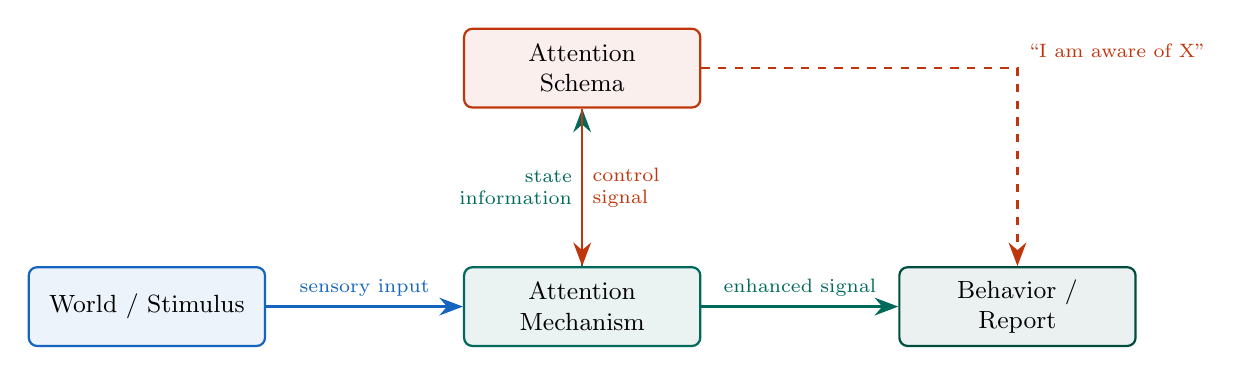
\begin{tikzpicture}[
    box/.style={rectangle, draw=#1, fill=#1!8, thick, minimum width=3cm, minimum height=1cm, font=\small, align=center, rounded corners=3pt},
    arr/.style={-{Stealth[length=3mm]}, thick},
    node distance=1.5cm,
  ]
  \node[box=defcolor] (world) {World / Stimulus};
  \node[box=mechcolor, right=2.5cm of world] (att) {Attention\\Mechanism};
  \node[box=principlecolor, above=2cm of att] (schema) {Attention\\Schema};
  \node[box=darkteal, right=2.5cm of att] (out) {Behavior /\\Report};

  \draw[arr, defcolor] (world) -- node[above, font=\scriptsize] {sensory input} (att);
  \draw[arr, mechcolor] (att) -- node[above, font=\scriptsize] {enhanced signal} (out);
  \draw[arr, mechcolor] (att) -- node[left, font=\scriptsize, align=right] {state\\information} (schema);
  \draw[arr, principlecolor] (schema) -- node[right, font=\scriptsize, align=left] {control\\signal} (att);
  \draw[arr, principlecolor, dashed] (schema) -| node[above right, font=\scriptsize] {``I am aware of X''} (out);
\end{tikzpicture}
\end{center}
\vspace{-2pt}
{\small\centering\textit{Figure: The attention-schema control loop. The schema monitors attention, controls it, and generates reports about awareness.}\par}

\subsection{Formal Model}

Let $\mathbf{a}(t)$ represent the state of attention (a vector describing which stimuli are being enhanced and by how much), and $\hat{\mathbf{a}}(t)$ represent the attention schema's estimate of the attentional state.

\begin{mathbox}
\vspace{-6pt}
\textbf{Attention dynamics:}
\begin{align}
  \tau_a \frac{d\mathbf{a}}{dt} &= -\mathbf{a} + \Phi\!\left(W_{\text{stim}}\, \mathbf{s}(t) + W_{\text{ctrl}}\, \mathbf{u}(\hat{\mathbf{a}}) + \boldsymbol{\eta}_a\right) \label{eq:att_dyn}
\end{align}
\textbf{Attention schema dynamics:}
\begin{align}
  \tau_s \frac{d\hat{\mathbf{a}}}{dt} &= -\hat{\mathbf{a}} + \Psi\!\left(W_{\text{obs}}\, \mathbf{a}(t) + W_{\text{prior}}\, \hat{\mathbf{a}} + \boldsymbol{\eta}_s\right) \label{eq:schema_dyn}
\end{align}
\textbf{Control policy:}
\begin{align}
  \mathbf{u}(\hat{\mathbf{a}}) &= \pi(\hat{\mathbf{a}},\; \mathbf{g}) \label{eq:control}
\end{align}
\vspace{-8pt}
\end{mathbox}

where:
\begin{itemize}[leftmargin=1.5em]
  \item $\mathbf{s}(t)$: stimulus input; $\mathbf{g}$: current goal
  \item $W_{\text{stim}}$: bottom-up stimulus-to-attention weights
  \item $W_{\text{ctrl}}$: control-to-attention weights (how the schema influences attention)
  \item $W_{\text{obs}}$: attention-to-schema observation weights
  \item $W_{\text{prior}}$: recurrent prior within the schema
  \item $\Phi, \Psi$: nonlinear activation functions
  \item $\boldsymbol{\eta}_a, \boldsymbol{\eta}_s$: noise terms
  \item $\pi$: control policy mapping schema state and goals to control signals
\end{itemize}

The critical feature: the schema $\hat{\mathbf{a}}$ is a \emph{model} of $\mathbf{a}$, not a copy. It is simplified ($\dim(\hat{\mathbf{a}}) \ll \dim(\mathbf{a})$ in general), noisy, and potentially distorted.

\section{The Schema as Dimensionality Reduction}

The attention mechanism is high-dimensional: it involves the gain of millions of neurons, their synchronization patterns, competitive interactions, etc. The schema compresses this into a low-dimensional representation:

\begin{mathbox}
\vspace{-8pt}
\[
  \hat{\mathbf{a}} = E(\mathbf{a}) \in \mathbb{R}^k, \qquad k \ll \dim(\mathbf{a})
\]
where $E : \mathbb{R}^n \to \mathbb{R}^k$ is an encoding function that extracts the essential features of the attentional state:
\begin{itemize}[leftmargin=1.5em]
  \item What object/location is attended ($\hat{\mathbf{a}}_{\text{target}}$)
  \item How strongly ($\hat{a}_{\text{intensity}} \in [0,1]$)
  \item In what modality ($\hat{\mathbf{a}}_{\text{modality}}$)
  \item With what certainty ($\hat{a}_{\text{confidence}}$)
\end{itemize}
\vspace{-6pt}
\end{mathbox}

The compression inevitably loses information. Specifically, the schema \emph{does not represent the mechanism of attention}---it represents only its functional properties. This is why, when the brain introspects, it finds ``awareness'' (an abstract functional property) rather than ``gain modulation and biased competition'' (the mechanism). The schema's content is the source of the ``explanatory gap.''

\section{Predictive Processing Formulation}

AST can be cast in the predictive processing framework:

\begin{mathbox}
\vspace{-6pt}
The attention schema minimizes \textbf{prediction error} about the attentional state:
\begin{align}
  \varepsilon_a(t) &= \mathbf{y}_a(t) - g(\hat{\mathbf{a}}(t)) \label{eq:pred_err}\\
  \dot{\hat{\mathbf{a}}} &= -\frac{\partial F_a}{\partial \hat{\mathbf{a}}} = D\hat{\mathbf{a}} + \frac{\partial g^T}{\partial \hat{\mathbf{a}}}\, \Pi_a\, \varepsilon_a \label{eq:schema_pp}
\end{align}
where $\mathbf{y}_a$ is the observed attentional signal, $g(\hat{\mathbf{a}})$ is the schema's prediction of what the attention signal should look like, $\Pi_a$ is the precision of the prediction error, and $F_a$ is the free energy for the attentional model.
\vspace{-4pt}
\end{mathbox}

The schema is updated to minimize the discrepancy between its predictions and the actual attentional state. This is exactly the same principle as the body schema (which minimizes prediction error about proprioceptive signals) and the forward model (which minimizes prediction error about sensory consequences of actions).

\section{A Bayesian Model of Awareness Attribution}

AST can be formalized as a \textbf{Bayesian inference} problem: given noisy observations of the attentional state, infer whether attention is directed at stimulus $X$:

\begin{mathbox}
\vspace{-8pt}
\[
  P(\text{attending to } X \mid \text{observations}) = \frac{P(\text{observations} \mid \text{attending to } X)\, P(\text{attending to } X)}{P(\text{observations})}
\]
\vspace{-10pt}
\end{mathbox}

The brain reports ``being aware of $X$'' when this posterior exceeds a threshold:
\[
  \text{``I am aware of } X\text{''} \iff P(\text{attending to } X \mid \text{observations}) > \theta
\]

This connects AST to the signal detection framework used in HOT: the ``awareness threshold'' is a criterion on the internal model's confidence about the attentional state.

\section{Social Extension: Modeling Others' Attention}

AST proposes that the same schema architecture is used to model \emph{other agents'} attention:

\begin{mathbox}
\vspace{-6pt}
\textbf{Self-awareness:}
\[
  \hat{\mathbf{a}}_{\text{self}}(t) = E_{\text{self}}\bigl(\mathbf{a}_{\text{self}}(t)\bigr)
\]
\textbf{Other-awareness (Theory of Mind):}
\[
  \hat{\mathbf{a}}_{\text{other}}(t) = E_{\text{social}}\bigl(\text{gaze direction, behavior, context of other agent}\bigr)
\]
Both use the same representational format---the attention schema template---applied to different targets (self vs.\ other).
\vspace{-4pt}
\end{mathbox}

This explains why the same brain regions (TPJ, mPFC, STS) are activated for both self-awareness and theory of mind: they use the same schema machinery.


% ══════════════════════════════════════════════════════════════
\chapter{Neural Implementation}
% ══════════════════════════════════════════════════════════════

\section{Candidate Brain Regions}

AST predicts that the attention schema is constructed in brain regions that: (a) receive information about the current state of attention, (b) maintain an ongoing model of attentional deployment, and (c) contribute to attentional control and social cognition.

\begin{mechbox}[Neural Substrates of the Attention Schema]
\begin{enumerate}[leftmargin=1.5em]
  \item \textbf{Temporoparietal junction (TPJ):} Strongly associated with theory of mind, attention reorienting, and self-other attribution. AST predicts TPJ constructs the attention schema.
  \item \textbf{Superior temporal sulcus (STS):} Processes social signals (gaze direction, biological motion) related to others' attention. Used for the social component of the schema.
  \item \textbf{Medial prefrontal cortex (mPFC):} Self-referential processing, mentalizing, default mode network. May maintain the self-directed attention schema.
  \item \textbf{Insular cortex:} Interoceptive awareness, subjective feelings. May contribute to the ``experiential'' quality attributed by the schema.
  \item \textbf{Intraparietal sulcus (IPS):} Priority maps for attention. Provides state information \emph{to} the schema.
\end{enumerate}
\end{mechbox}

\section{Graziano Lab Experimental Evidence}

\subsection{TMS Studies}

Graziano and colleagues (Webb \& Graziano, 2015) applied TMS to TPJ while subjects performed a task requiring awareness judgments:
\begin{itemize}[leftmargin=1.5em]
  \item TMS to TPJ disrupted awareness reports (subjects reported lower visibility) without affecting first-order perceptual performance ($d'$ preserved).
  \item This is consistent with TPJ constructing the attention schema: disrupting the schema impairs awareness reports while leaving the underlying attention mechanism intact.
\end{itemize}

\subsection{The ``Awareness Detector'' Paradigm}

Wilterson et al.\ (2021) developed a paradigm to study the brain's attribution of awareness:
\begin{itemize}[leftmargin=1.5em]
  \item Subjects viewed displays and reported whether they were ``aware'' of a stimulus.
  \item By manipulating stimulus properties independently of attentional engagement, they showed that awareness reports track the \emph{schema} (internal model of attention) rather than attention itself.
  \item Brain imaging identified TPJ, STS, and mPFC as regions whose activity correlated with awareness reports above and beyond measures of attention.
\end{itemize}

\section{The Default Mode Network Connection}

AST connects to the \textbf{default mode network} (DMN: mPFC, posterior cingulate, TPJ, lateral temporal cortex), which is active during:
\begin{itemize}[leftmargin=1.5em]
  \item Self-referential thought
  \item Theory of mind / mentalizing
  \item Mind-wandering and internal reflection
\end{itemize}

AST interprets the DMN as the network that maintains and updates the attention schema during rest. When the brain is not focused on an external task, it runs the attention schema in a ``default'' mode, modeling its own ongoing stream of attention---which we experience as the ``stream of consciousness.''


% ══════════════════════════════════════════════════════════════
\chapter{AST and the ``Hard Problem''}
% ══════════════════════════════════════════════════════════════

\section{How AST Addresses the Hard Problem}

AST's approach to the Hard Problem is distinctive: rather than trying to explain \emph{why} physical processes give rise to subjective experience, AST explains \emph{why the brain claims to have subjective experience}---and argues that, once this is explained, there is nothing left to explain.

\begin{principlebox}[AST's Dissolution of the Hard Problem]
\begin{enumerate}[leftmargin=1.5em]
  \item The brain has a model (the attention schema) that describes its own attention.
  \item This model attributes to itself properties like ``subjective experience,'' ``inner awareness,'' and ``qualia.''
  \item When the brain introspects, it reads the content of the schema and concludes: ``I have subjective experience that seems non-physical and mysterious.''
  \item The Hard Problem arises because we take this introspective report at face value: we assume that because the brain says it has non-physical experience, there must actually be non-physical experience.
  \item But the schema is a \emph{simplified model} that doesn't represent its own mechanism. The ``non-physical'' quality attributed by the schema is an artifact of the model's simplification, not a real property of the world.
  \item Therefore, the Hard Problem is a \textbf{consequence of the schema's incompleteness}, not a genuine metaphysical puzzle.
\end{enumerate}
\end{principlebox}

\section{Illusionism}

AST is closely aligned with \textbf{illusionism} in philosophy of mind:

\begin{definitionbox}[Illusionism (Frankish, 2016)]
\textbf{Illusionism} is the view that phenomenal consciousness (qualia, the ``what it is like'' quality) does not exist in the way we think it does. Our introspective impression that we have rich, non-physical subjective experience is a kind of \textbf{introspective illusion}---the brain \emph{represents} itself as having these properties, but the representation is not accurate.
\end{definitionbox}

AST provides a specific \emph{mechanistic} account of how this illusion arises: the attention schema is the source of the illusion. The schema tells the brain it has ``awareness''---a property that seems non-physical, private, and ineffable---but this is because the schema is a simplified model that doesn't include its own mechanistic basis.

\begin{notebox}[AST vs.\ Strong Illusionism]
AST does not deny that there is \emph{something} happening in the brain that we call consciousness. It denies that this something has the properties we intuitively attribute to it (non-physicality, ineffability, intrinsic subjectivity). Consciousness is real as an information structure (the schema), but it is not what it seems to itself.
\end{notebox}

\section{The Explanatory Gap Explained}

The ``explanatory gap'' (Levine, 1983)---the sense that no physical explanation can fully capture the nature of conscious experience---is explained by AST as follows:

\begin{enumerate}[leftmargin=2em]
  \item The attention schema describes attention using abstract, functional properties (``awareness,'' ``experience'') without representing the underlying mechanism.
  \item When we try to bridge the gap between the physical mechanism (neurons, synapses) and the schema's content (``awareness''), we find an unbridgeable gulf.
  \item But this gulf is not between the physical and the experiential---it is between the \emph{mechanism} and the \emph{model of the mechanism}. Of course the model doesn't contain the mechanism's details: that's what makes it a useful simplification.
  \item The explanatory gap is therefore an artifact of the schema's design, not evidence of a fundamental metaphysical divide.
\end{enumerate}


% ══════════════════════════════════════════════════════════════
\chapter{Predictions and Experimental Tests}
% ══════════════════════════════════════════════════════════════

\section{Specific Predictions}

\begin{predbox}[Testable Predictions of AST]
\begin{enumerate}[leftmargin=1.5em]
  \item \textbf{Dissociation between attention and awareness:} It should be possible to disrupt the attention schema (and thus awareness reports) while leaving the attention mechanism intact, and vice versa.
  \item \textbf{TPJ involvement in awareness:} Disrupting TPJ should impair awareness reports and theory-of-mind attributions, but not low-level attentional selection.
  \item \textbf{Shared substrates for self- and other-awareness:} The same brain regions (TPJ, mPFC, STS) should be active when attributing awareness to self and to others.
  \item \textbf{Schema errors produce awareness errors:} If the schema misrepresents the attentional state, the subject should misreport their awareness. This includes change blindness (attention shifts but schema doesn't update) and inattentional blindness (schema models no attention $\to$ no awareness report).
  \item \textbf{Gradations of awareness:} The schema should represent attention as graded (levels of awareness), not all-or-none, corresponding to the confidence of the internal model.
  \item \textbf{Artificial awareness:} A machine with an attention mechanism and an attention schema should exhibit the same behavioral signatures of ``awareness'' (reporting inner experience, attributing awareness to others, showing attention-awareness dissociations).
\end{enumerate}
\end{predbox}

\section{Evidence Supporting AST}

\subsection{Attention--Awareness Dissociations}

Multiple studies demonstrate the predicted dissociations:
\begin{itemize}[leftmargin=1.5em]
  \item \textbf{Kentridge et al.\ (1999, 2004):} Blindsight patient GY showed attentional cueing effects (faster responses for cued locations) in his blind field, even though he denied awareness. This shows attention without awareness---the mechanism works but the schema doesn't model it.
  \item \textbf{Koch \& Tsuchiya (2007):} Review documenting multiple cases of attention without awareness and awareness without (focused) attention.
  \item \textbf{Webb \& Graziano (2015):} TMS to TPJ disrupted awareness reports while preserving attentional performance.
\end{itemize}

\subsection{Shared Self--Other Mechanisms}

\begin{itemize}[leftmargin=1.5em]
  \item \textbf{Saxe \& Kanwisher (2003):} TPJ activates for both self-referential and other-referential mental state attributions.
  \item \textbf{Mitchell et al.\ (2005):} mPFC activity during judgments about self and similar others overlaps significantly.
  \item \textbf{Guterstam et al.\ (2019, 2021):} Showed that the same regions (TPJ, STS) track the attribution of awareness to both self and others, consistent with a shared attention schema.
\end{itemize}

\subsection{Schema Errors as Awareness Errors}

\begin{itemize}[leftmargin=1.5em]
  \item \textbf{Change blindness:} The schema fails to update when attention shifts during a disruption (blink, saccade), so the subject reports no change. The schema error produces an awareness error.
  \item \textbf{Inattentional blindness:} The schema models no attention to the unexpected stimulus $\to$ no awareness report, even though some processing occurs.
  \item \textbf{Phantom awareness / filling-in:} The schema ``fills in'' awareness for missing sensory input (blind spot, scotomas), creating awareness of something not actually attended.
\end{itemize}

\section{Artificial Consciousness: The Engineering Test}

AST provides a concrete engineering proposal: build a machine with:
\begin{enumerate}[leftmargin=2em]
  \item An attention mechanism (selective signal enhancement).
  \item An attention schema (internal model of the attention mechanism).
  \item Access to the schema for control and reporting.
\end{enumerate}

Such a machine should:
\begin{itemize}[leftmargin=1.5em]
  \item Report ``being aware of'' stimuli it is attending to.
  \item Show attention--awareness dissociations when the schema is disrupted.
  \item Attribute ``awareness'' to other agents using the same schema template.
  \item Exhibit ``subjective'' reports that mirror human introspective descriptions.
\end{itemize}

Graziano and colleagues have begun building computational implementations (Kelly et al., 2020; Wilterson \& Graziano, 2021) demonstrating some of these properties.


% ══════════════════════════════════════════════════════════════
\chapter{AST vs.\ Other Theories}
% ══════════════════════════════════════════════════════════════

\section{AST vs.\ Global Workspace Theory}

\begin{compbox}[Key Differences: AST vs.\ GWT]
\renewcommand{\arraystretch}{1.4}
\begin{tabular}{>{\raggedright}p{3cm} >{\raggedright}p{5.2cm} >{\raggedright\arraybackslash}p{4.8cm}}
  \toprule
  \textbf{Dimension} & \textbf{AST} & \textbf{GWT / GNWT} \\
  \midrule
  What is consciousness? & Brain's model of attention & Global broadcast \\
  Consciousness is\ldots & An internal model (schema) & An information-sharing event \\
  Key mechanism & Attention schema in TPJ/mPFC & Ignition in PFC-parietal \\
  Hard Problem & Dissolved (schema artifact) & Not directly addressed \\
  Attention $=$ awareness? & No (explicitly dissociable) & Closely linked (broadcast $\approx$ attention) \\
  Social cognition link & Central (shared schema) & Not emphasized \\
  Artificial consciousness & Engineering proposal & Possible but less specific \\
  \bottomrule
\end{tabular}
\end{compbox}

AST and GWT are compatible in some respects: the global broadcast mechanism could be the \emph{mechanism of attention} that the schema models. The schema adds an explanation of \emph{why} broadcast feels like something: because the brain models the broadcast and attributes experiential properties to it.

\section{AST vs.\ Integrated Information Theory}

\begin{compbox}[Key Differences: AST vs.\ IIT]
\renewcommand{\arraystretch}{1.4}
\begin{tabular}{>{\raggedright}p{3cm} >{\raggedright}p{5.2cm} >{\raggedright\arraybackslash}p{4.8cm}}
  \toprule
  \textbf{Dimension} & \textbf{AST} & \textbf{IIT} \\
  \midrule
  Ontological status & Consciousness is an informational model & Consciousness is $\Phi$ (fundamental) \\
  Hard Problem & Dissolved & Identity claim \\
  Panpsychism & No & Yes \\
  Key brain areas & TPJ, STS, mPFC & Posterior cortex \\
  Illusionism & Yes (consciousness is not what it seems) & No (consciousness is exactly $\Phi$) \\
  Qualia & Schema-attributed properties & Constellation structure \\
  \bottomrule
\end{tabular}
\end{compbox}

AST and IIT are fundamentally opposed: IIT says consciousness is real and irreducible; AST says consciousness is a model that misrepresents its own nature. IIT identifies consciousness with integrated information; AST identifies it with a specific internal model.

\section{AST vs.\ Higher-Order Theories}

\begin{compbox}[Key Differences: AST vs.\ HOT]
\renewcommand{\arraystretch}{1.4}
\begin{tabular}{>{\raggedright}p{3cm} >{\raggedright}p{5.2cm} >{\raggedright\arraybackslash}p{4.8cm}}
  \toprule
  \textbf{Dimension} & \textbf{AST} & \textbf{HOT / PRM} \\
  \midrule
  HOR type & Model of attention (schema) & Thought / monitoring of state \\
  Misrepresentation? & Central (schema is a caricature) & Possible but not central \\
  Neural substrate & TPJ / STS / mPFC & dlPFC / aPFC \\
  Metacognition & Schema-based self-monitoring & Higher-order representation \\
  What is modeled? & Attention specifically & Any mental state \\
  Evolutionary story & Detailed (social cognition) & Less developed \\
  Overlap & AST is a specific mechanistic version of HOT applied to attention \\
  \bottomrule
\end{tabular}
\end{compbox}

AST can be viewed as a \emph{specific type} of higher-order theory: the higher-order representation is specifically an internal model of attention. AST adds the body-schema analogy, the evolutionary story, the social cognition connection, and the illusionist interpretation.

\section{AST vs.\ Recurrent Processing Theory}

\begin{compbox}[Key Differences: AST vs.\ RPT]
\renewcommand{\arraystretch}{1.4}
\begin{tabular}{>{\raggedright}p{3cm} >{\raggedright}p{5.2cm} >{\raggedright\arraybackslash}p{4.8cm}}
  \toprule
  \textbf{Dimension} & \textbf{AST} & \textbf{RPT (Lamme)} \\
  \midrule
  Minimal NCC & Schema network (TPJ/mPFC) & Recurrent loops in sensory cortex \\
  PFC role & Essential (schema construction) & Not needed for P-consciousness \\
  Phenomenal overflow & No (awareness $=$ schema content) & Yes (Stage 2 is conscious) \\
  Attention role & Central (consciousness models it) & Not specifically modeled \\
  Illusionism & Yes & No (recurrence $=$ real experience) \\
  \bottomrule
\end{tabular}
\end{compbox}


% ══════════════════════════════════════════════════════════════
\chapter{Criticisms and Open Questions}
% ══════════════════════════════════════════════════════════════

\section{Common Critiques}

\textbf{Critique 1: AST explains away consciousness rather than explaining it.}

By treating consciousness as a ``model'' or ``illusion,'' AST seems to deny the reality of the most basic fact of existence: that we have subjective experiences. Critics argue that the very datum to be explained---the experience itself---is dismissed.

\emph{Response:} AST does not deny that something is happening when we are conscious. It denies that this something has the properties we intuitively attribute to it (non-physicality, ineffability). The attention schema is a real information structure in the brain that has real causal consequences. AST reinterprets, rather than eliminates, consciousness.

\textbf{Critique 2: The Hard Problem persists.}

Even if the attention schema explains why the brain \emph{claims} to have experience, it doesn't explain why there \emph{is} experience. The schema could exist without any ``inner light''---so why isn't the schema just an unconscious model?

\emph{Response:} AST argues this objection begs the question by assuming there is a separate ``inner light'' beyond the schema. If the schema is all there is, then asking why the schema ``has experience'' is like asking why a map ``has geography.'' The map doesn't have geography; it represents geography. Similarly, the schema doesn't ``have'' experience; it represents the organism as having experience. The apparent residual mystery is a consequence of taking the schema's content (``I have non-physical experience'') too literally.

\textbf{Critique 3: Attention and consciousness may not be as closely linked as AST assumes.}

Some researchers argue for cases of consciousness without attention (e.g., diffuse background awareness) that AST cannot accommodate.

\emph{Response:} AST acknowledges multiple forms of attention (focal, diffuse, feature-based, object-based). ``Background awareness'' may reflect diffuse attention modeled by the schema. The key is that the schema models \emph{some form of} attentional processing, not necessarily focal spatial attention.

\textbf{Critique 4: Lack of specific neural predictions.}

While AST implicates TPJ and mPFC, these regions are associated with many functions. The neural predictions are not specific enough to uniquely test AST.

\emph{Response:} Graziano's lab has begun generating more specific predictions, including TMS studies targeting TPJ and experiments dissociating attention from awareness reports. The engineering approach (building machines with attention schemas) provides another avenue for testing.

\textbf{Critique 5: Animal and infant consciousness.}

If consciousness requires a sophisticated internal model, do simple organisms with basic attentional mechanisms have any form of consciousness?

\emph{Response:} AST proposes a continuum: simple organisms may have rudimentary attention schemas (basic models of their own attentional priorities), producing rudimentary awareness. Full human-like consciousness requires the more elaborate schema that emerged with social cognition and language. The evolutionary stages outlined in Chapter~3 describe this gradient.

\section{Open Questions}

\begin{enumerate}[leftmargin=2em]
  \item \textbf{What is the minimal attention schema?} How simple can the model be and still produce something recognizable as awareness?
  \item \textbf{Can we measure the schema directly?} What neural signature would distinguish the attention schema from other forms of internal modeling?
  \item \textbf{How does the schema interact with emotion?} Emotional experiences seem different from perceptual awareness---does the schema model emotional attention differently?
  \item \textbf{What happens to the schema during sleep and anesthesia?} AST predicts the schema shuts down during unconsciousness, but the details are underspecified.
  \item \textbf{Can an artificial attention schema produce genuine awareness?} Or does it only produce the \emph{behavioral signature} of awareness? (AST would say these are the same thing.)
  \item \textbf{How does the schema handle the unity of consciousness?} We seem to have one unified awareness, but we attend to multiple things---how does the schema integrate?
  \item \textbf{Relationship to dreaming:} During dreaming, the schema may model internally generated ``attention,'' producing awareness of dream content. This is consistent with AST but requires formalization.
\end{enumerate}


% ══════════════════════════════════════════════════════════════
\chapter{Further Reading and References}
% ══════════════════════════════════════════════════════════════

\section*{Core AST Publications}
\begin{enumerate}[label={[\arabic*]}, leftmargin=2.5em]
  \item Graziano, M.\ S.\ A.\ (2013). \textit{Consciousness and the Social Brain}. Oxford University Press.
  \item Graziano, M.\ S.\ A.\ (2019). \textit{Rethinking Consciousness: A Scientific Theory of Subjective Experience}. W.\ W.\ Norton.
  \item Graziano, M.\ S.\ A.\ \& Kastner, S.\ (2011). Human consciousness and its relationship to social neuroscience: A novel hypothesis. \textit{Cognitive Neuroscience}, 2(2), 98--113.
  \item Graziano, M.\ S.\ A.\ (2016). Consciousness engineered. \textit{Journal of Consciousness Studies}, 23(11--12), 98--115.
  \item Webb, T.\ W.\ \& Graziano, M.\ S.\ A.\ (2015). The attention schema theory: a mechanistic account of subjective awareness. \textit{Frontiers in Psychology}, 6, 500.
\end{enumerate}

\section*{Experimental Evidence}
\begin{enumerate}[label={[\arabic*]}, leftmargin=2.5em, start=6]
  \item Guterstam, A., Kean, H.\ H., Webb, T.\ W., Kean, F.\ S., \& Graziano, M.\ S.\ A.\ (2019). Implicit model of other people's visual attention as an invisible, force-carrying beam projecting from the eyes. \textit{PNAS}, 116(1), 328--333.
  \item Wilterson, A.\ I.\ \& Graziano, M.\ S.\ A.\ (2021). The attention schema theory in a neural network agent: Controlling visuospatial attention using a descriptive model of attention. \textit{PNAS}, 118(33), e2102421118.
  \item Guterstam, A., Bio, B.\ J., Wilterson, A.\ I., \& Graziano, M.\ S.\ A.\ (2021). Temporo-parietal cortex involved in modeling one's own and others' attention. \textit{eLife}, 10, e63551.
  \item Kelly, Y.\ T., Webb, T.\ W., Meier, J.\ D., Arcaro, M.\ J., \& Graziano, M.\ S.\ A.\ (2014). Attributing awareness to oneself and to others. \textit{PNAS}, 111(13), 5012--5017.
\end{enumerate}

\section*{Attention and Social Cognition}
\begin{enumerate}[label={[\arabic*]}, leftmargin=2.5em, start=10]
  \item Desimone, R.\ \& Duncan, J.\ (1995). Neural mechanisms of selective visual attention. \textit{Annual Review of Neuroscience}, 18, 193--222.
  \item Koch, C.\ \& Tsuchiya, N.\ (2007). Attention and consciousness: two distinct brain processes. \textit{Trends in Cognitive Sciences}, 11(1), 16--22.
  \item Kentridge, R.\ W., Heywood, C.\ A., \& Weiskrantz, L.\ (2004). Spatial attention speeds discrimination without awareness in blindsight. \textit{Neuropsychologia}, 42(6), 831--835.
  \item Saxe, R.\ \& Kanwisher, N.\ (2003). People thinking about thinking people: the role of the temporo-parietal junction in ``theory of mind.'' \textit{NeuroImage}, 19(4), 1835--1842.
  \item Mitchell, J.\ P., Banaji, M.\ R., \& Macrae, C.\ N.\ (2005). The link between social cognition and self-referential thought in the medial prefrontal cortex. \textit{Journal of Cognitive Neuroscience}, 17(8), 1306--1315.
\end{enumerate}

\section*{Internal Models and Control Theory}
\begin{enumerate}[label={[\arabic*]}, leftmargin=2.5em, start=15]
  \item Wolpert, D.\ M., Ghahramani, Z., \& Jordan, M.\ I.\ (1995). An internal model for sensorimotor integration. \textit{Science}, 269(5232), 1880--1882.
  \item Graziano, M.\ S.\ A.\ \& Botvinick, M.\ M.\ (2002). How the brain represents the body: insights from neurophysiology and psychology. In \textit{Common Mechanisms in Perception and Action}, W.\ Prinz \& B.\ Hommel (Eds.), 136--157.
  \item Kalman, R.\ E.\ (1960). A new approach to linear filtering and prediction problems. \textit{Journal of Basic Engineering}, 82(1), 35--45.
\end{enumerate}

\section*{Illusionism and Philosophy}
\begin{enumerate}[label={[\arabic*]}, leftmargin=2.5em, start=18]
  \item Frankish, K.\ (2016). Illusionism as a theory of consciousness. \textit{Journal of Consciousness Studies}, 23(11--12), 11--39.
  \item Dennett, D.\ C.\ (1991). \textit{Consciousness Explained}. Little, Brown.
  \item Levine, J.\ (1983). Materialism and qualia: the explanatory gap. \textit{Pacific Philosophical Quarterly}, 64(4), 354--361.
  \item Chalmers, D.\ J.\ (1995). Facing up to the problem of consciousness. \textit{Journal of Consciousness Studies}, 2(3), 200--219.
\end{enumerate}

\section*{Theory Comparisons}
\begin{enumerate}[label={[\arabic*]}, leftmargin=2.5em, start=22]
  \item Seth, A.\ K.\ \& Bayne, T.\ (2022). Theories of consciousness. \textit{Nature Reviews Neuroscience}, 23, 439--452.
  \item Melloni, L., et al.\ (2021). Making the hard problem of consciousness easier. \textit{Science}, 372(6545), 911--912.
  \item Mashour, G.\ A., Roelfsema, P., Changeux, J.-P., \& Dehaene, S.\ (2020). Conscious processing and the global neuronal workspace hypothesis. \textit{Neuron}, 105(5), 776--798.
\end{enumerate}

\vfill
\begin{center}
  {\color{gray}\rule{0.4\textwidth}{0.5pt}}\\[8pt]
  {\small\color{gray}\itshape End of Document}
\end{center}

\end{document}
